\chapter{Drehungen, Spinoren und Farbsymmetrie}

\section{Drehungen als Gruppe}

Drehungen des Raums sind Symmetrien und wirken auf viele Arten von Objekten. Sie wirken auf starre Körper, Geschwindigkeitsvektoren, Vektorfelder und Quantenzustände. Ein gewöhnlicher Vektor ist der einfachste Ausgangspunkt, weil sich seine Transformation unmittelbar veranschaulichen lässt.

Drehungen lassen sich auch miteinander verknüpfen. Man dreht ein Objekt zunächst um eine Achse mit einem bestimmten Winkel und anschließend um eine zweite Achse mit einem zweiten Winkel. Die resultierende Orientierung entspricht einer einzelnen Drehung um eine dritte Achse mit einem dritten Winkel. Das Produkt zweier Drehungen ist also wieder eine Drehung.

Dieses Produkt ist eine Verknüpfung von Transformationen, keine Addition der beiden Achsenvektoren. Die erste Drehung verändert das Objekt, auf das die zweite wirkt. Wird \(R_1\) zuerst und \(R_2\) danach ausgeführt, schreibt man die zusammengesetzte Operation als \(R_2R_1\). Sie ist selbst ein \(R_3\), auch wenn es umständlich sein kann, die Achse und den Winkel von \(R_3\) zu bestimmen. Diese Abgeschlossenheit gegenüber der Verknüpfung ist der erste Grund, Drehungen als Gruppe und nicht bloß als Liste geometrischer Bewegungen aufzufassen.

Zunächst lässt sich eine einzelne Drehung geometrisch beschreiben. Dazu wählen wir einen Einheitsvektor \(\hat{\boldsymbol n}\) entlang der Drehachse und einen Winkel \(\theta\). Wir verwenden die Rechtsschraubenkonvention. Eine Linksdrehung um \(\theta\) lässt sich ebenso als Rechtsdrehung um \(-\theta\) oder als Rechtsdrehung um \(-\hat{\boldsymbol n}\) schreiben.

\begin{figure}[htbp]\centering
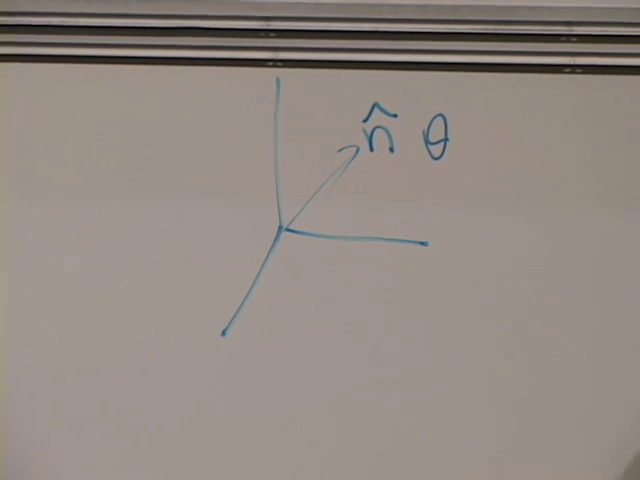
\includegraphics[width=0.58\textwidth]{lecture_03_figure_02.png}\caption{Eine Achse \(\hat{\boldsymbol n}\) und ein Winkel \(\theta\) legen eine räumliche Drehung fest.}\lectureframe{00:02:34}\end{figure}

Eine Richtung auf der Einheitskugel wird durch zwei Parameter festgelegt, etwa Länge und Breite. Der Drehwinkel um diese Richtung liefert einen dritten Parameter. Drehungen bilden daher eine dreiparametrige Familie. Die globalen Identifikationen, die durch Winkel entstehen, die sich um \(2\pi\) unterscheiden, lassen wir zunächst außer Acht; hier ist die lokale Parameterzahl entscheidend.

Die Beschreibung durch Achse und Winkel ist teilweise redundant. Eine Umkehrung der Achse zusammen mit einer Umkehrung des Winkels ergibt dieselbe Operation, und hinreichend große Winkel lassen sich modulo einer vollen Umdrehung reduzieren. Unberührt davon bleibt, dass eine Drehung in der Nähe der Identität durch drei stetig veränderliche Parameter beschrieben wird. Diese lokale Parameterzahl werden wir später mit der Zahl unabhängiger Parameter einer Matrixdarstellung vergleichen.

Die Gruppeneigenschaften lassen sich nun der Reihe nach überprüfen:
\begin{enumerate}\item \emph{Abgeschlossenheit.}Zwei aufeinanderfolgende Drehungen ergeben wieder eine Drehung.
\item \emph{Identität.}Nichts zu tun ist die Identitätsdrehung.
\item \emph{Inverse.}Eine Drehung um \(\theta\) um \(\hat{\boldsymbol n}\) wird durch eine Drehung um \(-\theta\) um dieselbe Achse rückgängig gemacht.
\item \emph{Assoziativität.}Für drei aufeinanderfolgende Drehungen gilt
\[
(R_1R_2)R_3=R_1(R_2R_3).
\]\end{enumerate}

Drehungen sind nicht kommutativ. Eine Drehung um die \(x\)-Achse, gefolgt von einer Drehung um die \(y\)-Achse, führt im Allgemeinen zu einer anderen Orientierung als dieselben beiden Operationen in umgekehrter Reihenfolge:
\begin{equation}
R_x(\alpha)R_y(\beta)\ne R_y(\beta)R_x(\alpha).
\end{equation}
Bei sehr kleinen Winkeln ist die Differenz von zweiter Ordnung. Deshalb können infinitesimale Drehungen beinahe kommutativ erscheinen. Die vollständige Gruppe ist dennoch nichtabelsch.

Die Nichtkommutativität lässt sich auch ohne Gleichungen überprüfen. Nehmen Sie ein Buch oder eine Schachtel und markieren Sie eine Seite als Vorderseite. Drehen Sie das Objekt zuerst um neunzig Grad um die \(x\)-Achse und dann um neunzig Grad um die \(y\)-Achse. Bringen Sie es wieder in die Ausgangsorientierung und vertauschen Sie die Reihenfolge. Die markierte Seite zeigt anschließend in eine andere Richtung. Bei kleinen Winkeln ist der Unterschied schwerer zu erkennen, aber er verschwindet nicht; er setzt bei dem Produkt der beiden kleinen Winkel ein.

\begin{classroomqa}\audiencequestion{Sind diese Drehungen nacheinander und nicht gleichzeitig ausgeführt?\lecturetimestamp{00:04:45}}\lecturerresponse{Ja. Die Gruppenmultiplikation bedeutet, dass eine Operation auf eine andere folgt. Gerade die Reihenfolge dieser aufeinanderfolgenden Drehungen kann die Kommutativität verletzen.}\end{classroomqa}

Dies ist unsere erste nichtabelsche Gruppe. Die spätere Anwendung betrifft nicht die Farbe eines gewöhnlichen Objekts, sondern die roten, grünen und blauen Farbzustände eines Quarks. Es handelt sich um ein internes System mit drei Zuständen, dessen interessante Transformationen die drei Farben miteinander mischen. Gewöhnliche Drehungen liefern ein anschauliches Beispiel dafür, wie eine kontinuierliche Gruppe durch Matrizen wirkt.

Eine Gruppe für sich genommen ist abstrakt. Um sie in der Physik zu verwenden, müssen wir angeben, auf welche Objekte sie wirkt. Eine {Darstellung} ordnet jedem Gruppenelement einen Operator oder eine Matrix zu, sodass die Multiplikation der Gruppenelemente durch die Multiplikation der zugeordneten Matrizen wiedergegeben wird. Verschiedene physikalische Objekte können unterschiedliche Darstellungen derselben Gruppe tragen. Vektoren, Spin-eins-Zustände und Spin-einhalb-Zustände liefern drei Beispiele.

\section{Die dreidimensionale Vektordarstellung}

Ein gewöhnlicher Vektor habe die Komponenten
\begin{equation}
\boldsymbol V=(V_x,V_y,V_z),\qquad V_i,\quad i=1,2,3.
\end{equation}
Man kann den physikalischen Vektor drehen und die Achsen festhalten oder die Koordinatenachsen drehen und den Vektor festhalten. Die Konventionen unterscheiden sich, doch in beiden Beschreibungen werden die Komponenten durch eine \(3\times3\)-Matrix gemischt. Für jedes Paar aus Achse und Winkel \((\hat{\boldsymbol n},\theta)\) schreiben wir
\begin{equation}
V_i'=R_{ij}(\hat{\boldsymbol n},\theta)V_j,
\label{eq:l3-vector-rotation}
\end{equation}
wobei über einen wiederholten Index summiert wird.

Der wiederholte Index \(j\) ist ein stummer Index. Gleichung~\eqref{eq:l3-vector-rotation} bedeutet ausgeschrieben
\begin{equation}
V_i'=R_{i1}V_1+R_{i2}V_2+R_{i3}V_3
\end{equation}
für jede Ausgangskomponente \(i\). Der freie Index \(i\) gibt an, welche Komponente berechnet wird; über den wiederholten Index \(j\) wird summiert, und er kann umbenannt werden, ohne die Gleichung zu ändern. Wenn man diese beiden Rollen auseinanderhält, lassen sich die meisten Indexfehler beim Argument zur Längenerhaltung vermeiden.

\begin{figure}[htbp]\centering
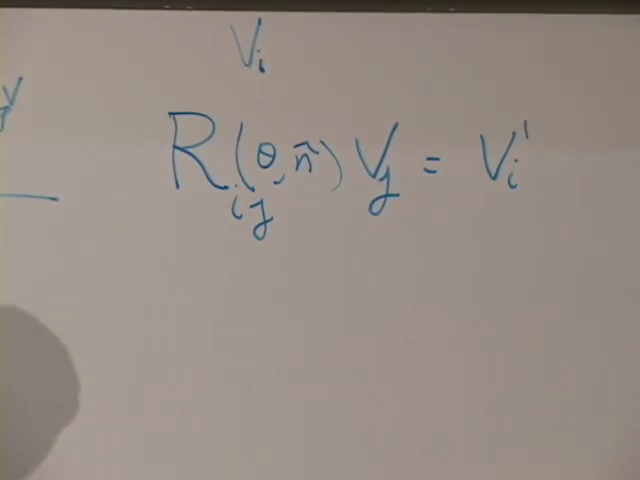
\includegraphics[width=0.68\textwidth]{lecture_03_figure_03.png}\caption{Eine Drehungsmatrix bildet die ursprünglichen Vektorkomponenten auf die gedrehten Komponenten ab.}\lectureframe{00:07:41}\end{figure}

Eine echte Drehung erhält die Länge. Vorerst sind sowohl \(V_i\) als auch \(R_{ij}\) reell, also gilt
\begin{equation}
V_i'V_i'=V_iV_i
\end{equation}
für jeden Vektor. Um die Bedingung an die Matrix sichtbar zu machen, schreiben wir dieselbe Transformation mit verschiedenen stummen Indizes:
\begin{equation}
V_i'=R_{ij}V_j,\qquad V_i'=R_{ik}V_k.
\end{equation}
Multiplikation und Summation über \(i\) ergeben
\begin{align}
V_i'V_i'
 &=R_{ij}V_jR_{ik}V_k\\
 &=R_{ij}R_{ik}V_jV_k.
\end{align}
Dies ist für jede Wahl von \(V\) nur dann gleich \(V_jV_j\), wenn
\begin{equation}
R_{ij}R_{ik}=\delta_{jk}.
\label{eq:l3-orthogonality-index}
\end{equation}
In Matrixschreibweise gilt
\begin{equation}
R^TR=\boldsymbol 1,
\label{eq:l3-orthogonal}
\end{equation}
und damit
\begin{equation}
R^{-1}=R^T.
\end{equation}
Die Transposition vertauscht lediglich Zeilen und Spalten.

Warum muss der Koeffizient \(\delta_{jk}\) sein? Unter der Summation setzt das Kronecker-Delta \(j=k\):
\begin{equation}
\delta_{jk}V_jV_k=V_1^2+V_2^2+V_3^2.
\end{equation}
Wenn \(R_{ij}R_{ik}\) von \(\delta_{jk}\) abwiche, würde sich die Länge in einer bestimmten Richtung oder durch einen bestimmten Kreuzterm \(V_jV_k\) ändern. Da die Gleichheit für jeden möglichen Vektor gelten muss und nicht nur für einen ausgewählten, muss der Matrixkoeffizient selbst der Einheitsmatrix entsprechen.

Gleichung~\eqref{eq:l3-orthogonal} ist die definierende Orthogonalitätsbedingung für diese reelle Matrixdarstellung. Die Matrixmultiplikation bildet die Multiplikationstabelle räumlicher Drehungen nach. Dies ist nicht die einzige Darstellung der Drehgruppe, sondern lediglich die am leichtesten zu veranschaulichende.

Die inverse Beziehung hat eine unmittelbare geometrische Bedeutung. Eine Drehung lässt sich rückgängig machen, ohne eine neue Matrixgleichung zu lösen: Man vertauscht Zeilen und Spalten. Wenn \(R_1\) und \(R_2\) zwei Drehungen darstellen, beschreibt \(R_2R_1\) ihre aufeinanderfolgende Wirkung und ist wiederum orthogonal. Die Matrixoperationen bewahren somit dieselben Eigenschaften Abgeschlossenheit, Identität, Inverses und Assoziativität, die wir geometrisch hergeleitet haben.

\section{Spin eins und die Vektordarstellung}

Die dreidimensionale Darstellung wirkt auch auf Quantenzustände. Ein Spin-eins-Teilchen hat drei mögliche Spinprojektionen:
\begin{equation}
m=+1,\quad 0,\quad -1.
\end{equation}
Sein Spinzustand ist daher eine dreikomponentige Spalte mit Wahrscheinlichkeitsamplituden. Wird das Teilchen gedreht oder die Orientierung eines Magnetfelds verändert, das die Spinachse festlegt, werden diese drei Amplituden durch eine dreidimensionale Darstellung der Drehgruppe miteinander gemischt.

Die Zahl der Spinzustände folgt der bekannten Regel \(2s+1\). Spin null hat einen Zustand, Spin einhalb zwei, Spin eins drei und Spin dreieinhalb vier. Die Dimension des Zustandsvektors hängt also vom Spin ab. Dieselbe physikalische Drehung muss durch Matrizen unterschiedlicher Größe dargestellt werden, wenn sie auf diese verschiedenen Zustandsräume wirkt.

Für ein Spin-eins-Teilchen wählen wir die Basis
\begin{equation}
\lvert 1,+1\rangle,qquad
\lvert 1,0\rangle,qquad
\lvert 1,-1\rangle.
\end{equation}
Ein Zustand ist
\begin{equation}
\lvert\psi\rangle
=c_{+}\lvert1,+1\rangle+c_0\lvert1,0\rangle+c_{-}\lvert1,-1\rangle.
\end{equation}
Durch eine Drehung des Versuchsaufbaus entsteht kein vierter Spinzustand; sie mischt lediglich die drei Koeffizienten \(c_+,c_0,c_-\) miteinander. Der zugehörige Drehoperator muss daher eine \(3\times3\)-Matrix sein.

Für Spin eins transformiert diese Darstellung wie ein gewöhnlicher räumlicher Vektor. Genau das bedeutet es, ein Spin-eins-Teilchen als \emph{Vektorteilchen} zu bezeichnen: Seine drei Spinamplituden und die drei Komponenten eines Vektors gehorchen demselben Drehungsgesetz. Der Quantenzustand muss dabei nicht als wörtlicher Pfeil aufgefasst werden; gemeint ist, wie sich seine Komponenten miteinander mischen.

Diese Entsprechung ist kein Zufall. Ein Dreivektor und ein Spin-eins-Zustand tragen äquivalente dreidimensionale Darstellungen der Drehgruppe. Die Bezeichnung {Vektorteilchen} fasst diese Transformationseigenschaft zusammen. Sie behauptet nicht, dass im Teilchen ein quantenmechanischer Polarisationszustand als winziger starrer Pfeil verborgen ist.

\section{Diskrete und kontinuierliche Symmetrien}

Bevor wir uns Spin einhalb zuwenden, ist es hilfreich, zwei grundlegende Arten von Gruppen zu unterscheiden. Eine Spiegelung ist ein einfaches diskretes Beispiel. Es gibt die Identität und die Spiegelung \(P\); entweder wird gespiegelt oder nicht. Dagegen hängt eine Phase
\begin{equation}
e^{i\phi}
\end{equation}
stetig von \(\phi\) ab, und eine räumliche Drehung hängt stetig von ihrer Achse und ihrem Winkel ab. Solche kontinuierlichen Gruppen nennt man \emph{Lie-Gruppen}, nach Sophus Lie; der Name wird \emph{Li} ausgesprochen. Im Mittelpunkt stehen kontinuierliche Symmetrien, doch auch diskrete Symmetrien bleiben wichtig.

Für die zweielementige Spiegelungsgruppe gilt
\begin{equation}
P^2=1.
\end{equation}
Zwischen \(1\) und \(P\) gibt es keine stetig einstellbare Stärke der Spiegelung. Eine Phasengruppe ist anders: Zwischen \(e^{i\phi_1}\) und \(e^{i\phi_2}\) liegen stetig unendlich viele weitere Phasen. Räumliche Drehungen haben denselben kontinuierlichen Charakter, sind aber anders als \(U(1)\) nichtabelsch.

Spin null liefert die einfachste Darstellung der Drehgruppe. Ein Spin-null-Zustand bleibt unter jeder Drehung unverändert; jedes Gruppenelement wird daher durch die eindimensionale Identität dargestellt:
\begin{equation}
D^{(0)}(R)=1.
\end{equation}
Die Gruppe selbst enthält weiterhin unendlich viele Drehungen; trivial ist lediglich ihre Darstellung auf dem Spin-null-Zustand.

Diese Unterscheidung zwischen einer Gruppe und einer ihrer Darstellungen ist wesentlich. Die Drehgruppe reduziert sich nicht auf eine Gruppe mit nur einem Element, wenn sie auf einen Skalar wirkt. Vielmehr wird jedes ihrer Elemente auf diesem bestimmten Skalarzustand durch dieselbe Zahl \(1\) dargestellt.

\section{Ein allgemeiner Spin-einhalb-Zustand}

Ein Spin-einhalb-System hat zwei Basiszustände. Bezogen auf eine gewählte \(z\)-Achse gilt
\begin{equation}
\lvert\uparrow\rangle=
\begin{pmatrix}1\\0\end{pmatrix},
\qquad
\lvert\downarrow\rangle=
\begin{pmatrix}0\\1\end{pmatrix}.
\end{equation}
Ein allgemeiner Zustand ist ein zweikomponentiger Spinor:
\begin{equation}
\lvert\psi\rangle=
\begin{pmatrix}\alpha_1\\\alpha_2\end{pmatrix},
\qquad
|\alpha_1|^2+|\alpha_2|^2=1.
\label{eq:l3-spinor}
\end{equation}
Die Einträge sind komplex. Für \((\alpha_1,\alpha_2)=(1,0)\) ist der Spin nach oben gerichtet, für \((0,1)\) nach unten. Eine allgemeine normierte Linearkombination beschreibt einen Spin, der entlang einer anderen Richtung polarisiert ist.

Die Begriffe {auf} und {ab} haben erst dann eine Bedeutung, wenn eine Achse gewählt wurde. Hier ist dies \(z\). Eine andere Messachse hat ein anderes Paar von Basiszuständen, und ein Zustand mit eindeutigem Spin nach oben entlang einer Achse erscheint in einer anderen Basis im Allgemeinen als Überlagerung. Eine Drehung des physikalischen Spins oder der Bezugsachsen ändert die Koeffizienten entsprechend.

Zwei komplexe Amplituden enthalten vier reelle Parameter. Durch die Normierung fällt einer weg; ein weiterer entfällt, weil die globale Phase physikalisch irrelevant ist. Es bleiben zwei reelle Parameter. Genau so viele werden benötigt, um eine Richtung auf einer Kugel festzulegen. Um Drehungen zu untersuchen, müssen wir die explizite Abbildung zwischen \((\alpha_1,\alpha_2)\) und dieser Richtung nicht herleiten.

Die globale Phase wird herausdividiert, weil
\begin{equation}
\begin{pmatrix}\alpha_1\\\alpha_2\end{pmatrix}
\quad\hbox{and}\quad
e^{i\chi}
\begin{pmatrix}\alpha_1\\\alpha_2\end{pmatrix}
\end{equation}
denselben physikalischen Strahl darstellen. Die Normierung legt die Gesamtwahrscheinlichkeit fest, nicht eine Richtung im gewöhnlichen euklidischen Raum. Nach beiden Identifikationen lassen sich die verbleibenden zwei Parameter als Polar- und Azimutwinkel der Spinpolarisationsrichtung auffassen.

Bei einer Drehung des Spins wird sein Zustand zu
\begin{equation}
\alpha_i'=U_{ij}\alpha_j,
\qquad
\begin{pmatrix}\alpha_1'\\\alpha_2'\end{pmatrix}
=
\begin{pmatrix}
U_{11}&U_{12}\\
U_{21}&U_{22}
\end{pmatrix}
\begin{pmatrix}\alpha_1\\\alpha_2\end{pmatrix}.
\label{eq:l3-spinor-transform}
\end{equation}
Räumliche Drehungen besitzen also eine zweidimensionale Matrizendarstellung, die auf Spinoren wirkt. Diese Darstellung weist eine globale Zweideutigkeit auf, auf die wir später zurückkommen; lokal haben die Matrizen die Transformationseigenschaften, die wir im Folgenden benötigen.

Das transformierte Paar \((\alpha_1',\alpha_2')\) muss wiederum einen möglichen Quantenzustand ergeben. Die erste Frage zu \(U\) betrifft daher nicht die explizite Formel für Achse und Winkel, sondern die Bedingung, dass die Normierung jedes Eingangsspinors erhalten bleibt.

\section{Wahrscheinlichkeitserhaltung und unitäre Matrizen}

Eine Drehung muss einen normierten Zustand auf einen anderen normierten Zustand abbilden:
\begin{equation}
\alpha_i^*\alpha_i=\alpha_i'^*\alpha_i'=1.
\end{equation}
Einsetzen von Gleichung~\eqref{eq:l3-spinor-transform} ergibt
\begin{align}
\alpha_i'^*\alpha_i'
 &=(U_{ij}\alpha_j)^*(U_{ik}\alpha_k)\\
 &=\alpha_j^*U_{ij}^*U_{ik}\alpha_k.
\end{align}
Das Analogon zur Bedingung für reelle Vektoren lautet daher
\begin{equation}
(U^T)^*U=\boldsymbol 1.
\end{equation}
Die Transposition zusammen mit komplexer Konjugation ist die hermitesche Konjugation:
\begin{equation}
U^\dagger=(U^T)^*,
\end{equation}
Somit lautet die Bedingung für den Erhalt der Normierung
\begin{equation}
U^\dagger U=\boldsymbol 1.
\label{eq:l3-unitarity}
\end{equation}

Die zusätzliche komplexe Konjugation ist die einzige wesentliche Änderung gegenüber der Rechnung mit reellen Vektoren. Für einen reellen Vektor ist \(V_iV_i\) eine Länge. Für einen Spinor ist \(\alpha_i^*\alpha_i\) eine Wahrscheinlichkeit. Komplexe Konjugation ist nötig, damit diese Wahrscheinlichkeit reell und nichtnegativ ist; deshalb tritt an die Stelle der Transposition die hermitesche Konjugation.

Gleichung~\eqref{eq:l3-unitarity} liefert unmittelbar auch die inverse Matrix:
\begin{equation}
U^{-1}=U^\dagger.
\end{equation}
Die inverse Drehung erhält also dieselbe Wahrscheinlichkeitsnorm. Wie bei gewöhnlichen Drehmatrizen bleibt auch ein Produkt unitärer Matrizen unitär, sodass die Darstellung die Gruppenmultiplikation respektiert.

\begin{figure}[htbp]\centering
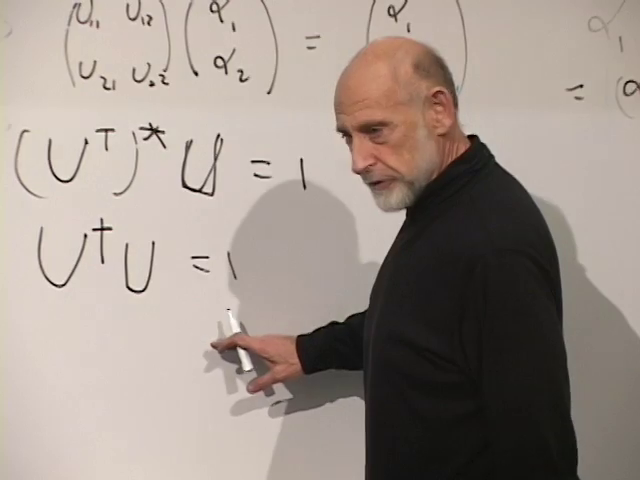
\includegraphics[width=0.62\textwidth]{lecture_03_figure_04.png}\caption{Die Spinordrehungsmatrix erfüllt \(U^\dagger U=\boldsymbol 1\).}\lectureframe{00:27:41}\end{figure}

Matrizen, die Gleichung ~\eqref{eq:l3-unitarity} erfüllen, sind unitär. Eine allgemeine komplexe \(2\times2\)-Matrix wird durch acht reelle Parameter beschrieben. Die Unitarität ist eine Matrixgleichung für \(2\times2\)-Matrizen, die vier unabhängige reelle Bedingungen liefert; damit bleiben vier Parameter. Eine räumliche Drehung hat nur drei. Eine weitere Einschränkung ist nötig, um die Spinordarstellung der Drehungen aus der Gesamtheit von \(U(2)\) herauszuheben.

Die vier Bedingungen lassen sich auch verstehen, indem man die beiden Spalten von \(U\) als zwei komplexe Vektoren auffasst. Jede Spalte muss die Norm eins haben, was zwei reelle Bedingungen ergibt. Außerdem müssen die Spalten orthogonal sein, was einer komplexen oder zwei reellen Bedingungen entspricht. Insgesamt sind es also vier. Wie sich herausstellen wird, ist der verbleibende vierte Parameter in \(U(2)\) eine globale Determinantenphase und keine neue räumliche Drehung.

\section{Determinante eins und \texorpdfstring{\(SU(2)\)}{SU(2)}}

Die zusätzliche Bedingung lautet
\begin{equation}
\det U=1.
\label{eq:l3-det-one}
\end{equation}
Sie ist mit der Gruppenmultiplikation verträglich, denn
\begin{equation}
\det(AB)=\det A\,\det B.
\end{equation}
Das Produkt zweier unitärer Matrizen mit Determinante eins hat wiederum Determinante eins, und auch die Identität hat Determinante eins. Diese Matrizen bilden eine abgeschlossene Untergruppe.

Auch die Inverse gehört zu dieser Untergruppe. Wenn \(\det U=1\), dann gilt
\begin{equation}
\det U^{-1}=\frac{1}{\det U}=1.
\end{equation}
Die Bedingung Determinante eins entfernt also weder die Identität noch stört sie die Abgeschlossenheit oder führt zum Verlust der Inversen. Sie legt konsistent eine Gruppe mit einem kontinuierlichen Parameter weniger fest.

Aus der Unitarität folgt allein
\begin{equation}
\det(U^\dagger U)=
(\det U)^*\det U
=|\det U|^2=1.
\end{equation}
Sie erzwingt nicht, dass \(\det U\) gleich \(+1\) oder \(-1\) ist. Die Determinante einer allgemeinen unitären Matrix kann eine beliebige Phase sein:
\begin{equation}
\det U=e^{i\phi},
\qquad
\det U^\dagger=e^{-i\phi}.
\end{equation}
Bedingung~\eqref{eq:l3-det-one} legt diese ansonsten freie Phase fest und entfernt einen reellen Parameter.

\begin{classroomqa}\audiencequestion{Erzwingt \(U^\dagger U=\boldsymbol 1\) ohne die Bedingung Determinante eins, dass \(\det U^\dagger\) gleich \(\det U\) oder nur \(+1\) oder \(-1\) ist?\lecturetimestamp{00:31:21}}\lecturerresponse{Nein. Die beiden Determinanten sind komplex konjugiert. Sie können \(e^{i\phi}\) und \(e^{-i\phi}\) sein; ihr Produkt ist dann eins. Die Einschränkung auf die spezielle unitäre Gruppe legt anschließend beide auf eins fest.}\end{classroomqa}

Die unitären \(n\times n\)-Matrizen bilden \(U(n)\). Für \(n=1\) ist eine unitäre Matrix einfach die Phase \(e^{i\phi}\); somit ergibt sich \(U(1)\). Die Untergruppe mit Determinante eins heißt \emph{spezielle unitäre Gruppe}:
\begin{equation}
SU(n)=\{U\in U(n):\det U=1\}.
\end{equation}
Auf den zweikomponentigen Spinor wirkt \(SU(2)\), eine dreiparametrige Gruppe.

Die Bezeichnung hält beide Einschränkungen fest: \(U\) steht für unitär, während \(S\) speziell bedeutet, also Determinante eins. Diese speziellen unitären Gruppen treten immer wieder auf, weil sie ein komplexes Skalarprodukt erhalten und zugleich die unabhängige globale Phase der Determinante ausschließen.

Lokal hat \(SU(2)\) dieselbe Drehungsalgebra und Multiplikationsstruktur, die für Drehungen von Spin-einhalb-Zuständen nötig sind. Global muss man die zuvor zurückgestellte Feinheit berücksichtigen: \(SU(2)\) ist die zweifache Überlagerung der gewöhnlichen Drehgruppe \(SO(3)\), sodass jeweils zwei Elemente von \(SU(2)\) einer räumlichen Drehung entsprechen. \editorialnote{Die Formulierung mit der zweifachen Überlagerung präzisiert die im Ausgangstext erwähnte, aber nicht ausgeführte Zweideutigkeit.}

\section{Infinitesimale Drehungen und Pauli-Matrizen}

\begin{classroomqa}\audiencequestion{Wie kommen die Spinmatrizen oder Pauli-Matrizen in diese Konstruktion?\lecturetimestamp{00:33:16}}\lecturerresponse{Sie treten auf, wenn man ein Gruppenelement betrachtet, das sehr nahe an der Identität liegt und einer Drehung um einen sehr kleinen Winkel entspricht. Sie sind die Erzeugenden dieser infinitesimalen Drehungen.}\end{classroomqa}

Wir beginnen mit
\begin{equation}
U=\boldsymbol 1+\epsilon M+O(\epsilon^2),
\label{eq:l3-small-u-anti}
\end{equation}
wobei \(\epsilon\) reell und klein ist. Dann gilt
\begin{equation}
U^\dagger=\boldsymbol 1+\epsilon M^\dagger+O(\epsilon^2),
\end{equation}
und aus der Unitarität folgt
\begin{align}
U^\dagger U
 &=\boldsymbol 1+\epsilon(M^\dagger+M)+O(\epsilon^2).
\end{align}
In erster Ordnung erhalten wir
\begin{equation}
M^\dagger=-M.
\end{equation}
Die Matrix \(M\) in Gleichung~\eqref{eq:l3-small-u-anti} ist also antihermitesch.

Es werden nur Terme linear in \(\epsilon\) beibehalten. Das Produkt \(\epsilon^2M^\dagger M\) wird vernachlässigt, weil es von zweiter Ordnung ist. Darin liegt der Vorteil, nahe an der Identität zu arbeiten: Nichtlineare Gruppenbedingungen werden zu linearen Bedingungen an ihre Erzeugenden.

Praktischer ist es, den Faktor \(i\) auszuklammern:
\begin{equation}
U=\boldsymbol 1+i\epsilon H+O(\epsilon^2).
\label{eq:l3-small-u-herm}
\end{equation}
Durch komplexe Konjugation wird \(i\) zu \(-i\), also gilt
\begin{equation}
U^\dagger=\boldsymbol 1-i\epsilon H^\dagger+O(\epsilon^2).
\end{equation}
Nun ist
\begin{equation}
U^\dagger U
=\boldsymbol 1+i\epsilon(H-H^\dagger)+O(\epsilon^2),
\end{equation}
und die Unitarität in erster Ordnung verlangt
\begin{equation}
H^\dagger=H.
\end{equation}
Wenn der Faktor \(i\) ausgeklammert ist, ist die Erzeugende hermitesch.

Die Multiplikation mit \(i\) ändert nicht, welche infinitesimalen Matrizen zulässig sind; sie ändert lediglich die Konvention zur Benennung der Erzeugenden. In der Physik wählt man gewöhnlich hermitesche Erzeugende, weil ihre Eigenwerte reell sind und die zugehörigen Observablen wie der Drehimpuls hermitesch sind.

Die Bedingung Determinante eins erzwingt Spurfreiheit\editorialnote{Bei der mündlichen Entwicklung der Determinante werden die Indizes kurzzeitig falsch wiedergegeben. Der korrigierte lineare Term lautet \(A_{11}+A_{22}=\operatorname{tr}A\); Produkte der Nichtdiagonalelemente beginnen erst in quadratischer Ordnung.}. Für eine kleine \(2\times2\)-Matrix \(A\) gilt
\begin{equation}
\det(\boldsymbol 1+A)
=
\det
\begin{pmatrix}
1+A_{11}&A_{12}\\
A_{21}&1+A_{22}
\end{pmatrix}.
\end{equation}
Entwickelt man die Determinante, erhält man
\begin{align}
\det(\boldsymbol 1+A)
 &=(1+A_{11})(1+A_{22})-A_{12}A_{21}\\
 &=1+A_{11}+A_{22}+O(A^2)\\
 &=1+\operatorname{tr}A+O(A^2).
\end{align}
Wenden wir dies auf \(A=i\epsilon H\) an, folgt
\begin{equation}
\det U=1+i\epsilon\,\operatorname{tr}H+O(\epsilon^2).
\end{equation}
Daher verlangt \(\det U=1\)
dass
\begin{equation}
\operatorname{tr}H=0.
\end{equation}
Die Spurbedingung entfernt genau die zur Einheitsmatrix proportionale Erzeugende. Eine allgemeine hermitesche \(2\times2\)-Matrix hat vier reelle Parameter: zwei reelle Diagonaleinträge und einen komplexen Nebendiagonaleintrag. Ihre Spur legt eine reelle Kombination fest, sodass drei Parameter übrig bleiben. Das entspricht den drei Achsen, um die eine infinitesimale räumliche Drehung erfolgen kann.

Die infinitesimalen Erzeugenden von \(SU(2)\) sind somit spurfrei-hermitesche \(2\times2\)-Matrizen. Die drei Pauli-Matrizen bilden eine Basis:
\begin{equation}
\begin{aligned}
\sigma_x&=
\begin{pmatrix}0&1\\1&0\end{pmatrix},
&
\sigma_y&=
\begin{pmatrix}0&-i\\i&0\end{pmatrix},
\\[0.4em]
\sigma_z&=
\begin{pmatrix}1&0\\0&-1\end{pmatrix}.
\end{aligned}
\end{equation}
Jede Erzeugende lässt sich schreiben als
\begin{equation}
H=a_x\sigma_x+a_y\sigma_y+a_z\sigma_z.
\end{equation}
Eine kleine Drehung um die \(x\)-Achse wählt \(\sigma_x\) aus, eine um die \(y\)-Achse \(\sigma_y\), und eine Drehung um eine beliebige andere Achse wählt die entsprechende Linearkombination aus. In Einheiten mit \(\hbar=1\) lauten die Spinoperatoren
\begin{equation}
S_i=\frac{\sigma_i}{2}.
\end{equation}

Eine Achse, die beispielsweise genau zwischen \(x\) und \(y\) liegt, verwendet eine Erzeugende proportional zu
\begin{equation}
\frac{\sigma_x+\sigma_y}{\sqrt2}.
\end{equation}
Die Richtung des Koeffizientenvektors \((a_x,a_y,a_z)\) legt die Drehachse fest, während sein Betrag zusammen mit \(\epsilon\) den kleinen Winkel bestimmt. So hängen die aus den Drehimpulskommutatoren bekannten Spinmatrizen mit endlichen Drehoperatoren zusammen. Insbesondere kodieren
\begin{equation}
[S_x,S_y]=iS_z
\end{equation}
und die zyklisch vertauschten Beziehungen die bereits geometrisch erkannte Nichtkommutativität. Die übliche Formel für eine endliche Drehung erhält man, indem man die infinitesimale Erzeugende exponentiert\editorialnote{Die Exponentialformel für endliche Drehungen ist die übliche Fortsetzung der infinitesimalen Konstruktion; die Quelle leitet nur die Bedingungen an die Erzeugenden und ihre Pauli-Matrix-Basis her.}:
\begin{equation}
U(\hat{\boldsymbol n},\theta)
=\exp\left(-\frac{i\theta}{2}\,
\hat{\boldsymbol n}\cdot\boldsymbol\sigma\right).
\end{equation}\section{Ein dreidimensionaler Farbraum}

Die Kombination von Darstellungen kann warten. Wir verlassen nun den räumlichen Spin und wenden uns wieder der Quarkfarbe zu. Ein Quark hat weiterhin Spin einhalb, doch seine Farbe ist ein davon unabhängiger Freiheitsgrad mit drei Zuständen:
\begin{equation}
\lvert r\rangle,\qquad
\lvert g\rangle,\qquad
\lvert b\rangle.
\end{equation}
Ein allgemeiner Farbenzustand ist
\begin{equation}
\begin{aligned}
\lvert q\rangle_{\mathrm{color}}
={}&
\alpha_r\lvert r\rangle
+\alpha_g\lvert g\rangle
+\alpha_b\lvert b\rangle,
\\
&|\alpha_r|^2+|\alpha_g|^2+|\alpha_b|^2=1.
\end{aligned}
\end{equation}
Äquivalent dazu gilt
\begin{equation}
q=
\begin{pmatrix}
\alpha_r\\
\alpha_g\\
\alpha_b
\end{pmatrix}.
\end{equation}
Die Betragsquadrate sind die Wahrscheinlichkeiten für Rot, Grün und Blau in einer gewählten Farbbasis. Dieselbe Tripletnotation kann auch drei Quarkfeldoperatoren zu einer Spalte zusammenfassen:
\begin{equation}
\psi=
\begin{pmatrix}
\psi_r\\
\psi_g\\
\psi_b
\end{pmatrix}.
\end{equation}

Spin und Farbe müssen gedanklich getrennt bleiben. Der Spinindex gibt an, wie der Zustand unter Drehungen des physikalischen Raums transformiert. Der Farbindex gibt an, wie er sich unter einer internen Symmetrie transformiert, die das Labor nicht dreht. Ein Quarkzustand trägt beide Indizes, obwohl wir den Spin in der vorliegenden Diskussion ausblenden, um uns auf die Farbe zu konzentrieren.

Drei Feldoperatoren in eine Spalte zu schreiben, ist mehr als bloße Buchführung. So lässt sich die Symmetrie mit einer einzigen Matrixgleichung formulieren. Eine Transformation kann ein rotes Feld in eine Linearkombination roter, grüner und blauer Felder überführen, so wie eine räumliche Drehung eine Vektorkomponente in eine Linearkombination der anderen Komponenten überführt.

Zunächst kann man sich diskrete Transformationen vorstellen, die zwei Farben vertauschen. Die größere Symmetrie umfasst kontinuierliche Mischungen aller drei Farben. Bei einer einfachen Vertauschungsmatrix ist möglicherweise eine zusätzliche Phase nötig, damit ihre Determinante eins ist; mit dieser Phase ist die Vertauschung in die spezielle unitäre Gruppe eingebettet.

Für zwei Basiszustände wird die unveränderte Vertauschung dargestellt durch
\begin{equation}
X=
\begin{pmatrix}0&1\\1&0\end{pmatrix},
\qquad
\det X=-1.
\end{equation}
Multipliziert man die gesamte Matrix mit \(i\), erhält man
\begin{equation}
\det(iX)=i^2\det X=1.
\end{equation}
Mit einer passend gewählten Phase kann die diskrete Vertauschung somit als bestimmtes Element der größeren kontinuierlichen Gruppe auftreten.

\begin{classroomqa}\audiencequestion{Hat eine Matrix, die lediglich zwei Basiszustände vertauscht, für \(SU(2)\) die falsche Determinante?\lecturetimestamp{00:43:46}}\lecturerresponse{Die unveränderte Vertauschung hat die Determinante \(-1\). Ein geeigneter Faktor \(i\) liefert eine Darstellung mit Determinante eins, sodass sich die Vertauschung in die kontinuierlichen speziellen unitären Transformationen einordnen lässt.}\end{classroomqa}

\section{\texorpdfstring{\(SU(3)\)}{SU(3)} und die acht Farberzeugenden}

Die kontinuierliche Farbtransformation lautet
\begin{equation}
\begin{aligned}
q'&=Uq,
&
U^\dagger U&=\boldsymbol 1,
\\
\det U&=1,
&
U&\in SU(3).
\end{aligned}
\label{eq:l3-su3-action}
\end{equation}
Mathematisch ist dies dieselbe spezielle unitäre Konstruktion wie bei den Spinoren, doch nun ist \(U\) eine \(3\times3\)-Matrix. Es handelt sich nicht um eine Drehung des physikalischen Raums, sondern um eine Drehung im internen Farbraum.

Die Unitarität erhält die Normierung des Farbenzustands:
\begin{equation}
q^\dagger q
=|\alpha_r|^2+|\alpha_g|^2+|\alpha_b|^2.
\end{equation}
Die Bedingung Determinante eins entfernt die Richtung der gemeinsamen Phase \(U(1)\) aus der kontinuierlichen Mischung. Die resultierenden Matrizen können einfache Vertauschungen, relative Phasenänderungen und echte kontinuierliche Überlagerungen bewirken und bleiben dabei Elemente einer einzigen abgeschlossenen Gruppe.

Die Parameterzahl ergibt sich unmittelbar. Eine komplexe \(3\times3\)-Matrix hat neun komplexe Einträge, also achtzehn reelle Parameter. Die Matrixgleichung \(U^\dagger U=\boldsymbol 1\) liefert neun reelle Bedingungen. Die Determinante eins entfernt einen weiteren Parameter:
\begin{equation}
\dim SU(3)=18-9-1=8.
\end{equation}
Damit hat \(SU(3)\) acht unabhängige infinitesimale Erzeugende.

Die neun reellen Unitaritätsbedingungen lassen sich wiederum anhand der Spalten von \(U\) verstehen. Jede der drei komplexen Spalten muss die Norm eins haben, und jedes Spaltenpaar muss orthogonal sein. Diese Bedingungen entfernen neun der ursprünglich achtzehn reellen Parameter. Die Determinantenphase entfernt den zehnten; acht bleiben übrig. Dies ist das Analogon für drei Zustände zur Zählung \(8-4-1=3\) für \(SU(2)\).

Das Auftreten der Acht ist derselbe Sachverhalt, aus dem letztlich auch die acht Gluonenarten hervorgehen. Die Aussage, es gebe keine neun Gluonen, weil die Determinantenbedingung eine Richtung entfernt habe, ist lediglich eine Gedächtnisstütze. Genauer zerfallen die neun Farb-Antifarb-Matrizen in eine farbsinguläre Richtung, die proportional zur Einheitsmatrix ist, und acht spurfreie Richtungen. Die acht spurfreien Generatoren bilden die adjungierte Farbstruktur, die von den Gluonen der QCD getragen wird.\editorialnote{Die Formulierung als Singulett plus Oktett ist die standardmäßige präzise Fassung der bewusst heuristischen Determinantenbemerkung in der Quelle; die Konstruktion des Eichfeldes wird später behandelt.}

An dieser Stelle ist der Zusammenhang mit den acht Gluonen ein Hinweis, noch keine vollständige Herleitung. Um Eichbosonen zu erhalten, muss man die Farbsymmetrie zu einer lokalen Symmetrie machen und die kompensierenden Felder bestimmen. Die Parameterzählung hat bereits gezeigt, dass es acht unabhängige Richtungen gibt, in denen eine \(SU(3)\)-Farbtransformation von der Identität abweichen kann.

\section{Die Farbsymmetrie schränkt die QCD ein}

Die grundlegende Aussage über die Symmetrie lautet, dass die Physik unter der Farbtransformation in Gleichung~\eqref{eq:l3-su3-action} invariant ist. Dies ist die zentrale innere Symmetrie der Quantenchromodynamik. Die Mischung der Farbkomponenten ist formal analog zur Mischung von Spin-up- und Spin-down-Amplituden; diese Spinortransformationen wiederum stehen in Beziehung zu Drehungen räumlicher Richtungen. Die drei Räume dürfen jedoch nicht miteinander verwechselt werden.

Farbe als Symmetrie zu bezeichnen bedeutet, dass eine Änderung der Farbbasis die physikalischen Vorhersagen nicht verändert. Rot, Grün und Blau sind zweckmäßige Bezeichnungen für drei Basisvektoren, keine beobachtbaren Pigmente. Eine gleichzeitige \(SU(3)\)-Drehung der Farbkomponenten muss die Form der Gesetze unverändert lassen. Diese Invarianz ist kein optionales ästhetisches Merkmal, sondern das Ordnungsprinzip der QCD.

Die Symmetrie schränkt die Lagrange-Dichte ein. Im früheren \(U(1)\)-Beispiel führte die Invarianz unter einer gemeinsamen Phasentransformation dazu, dass zulässige Terme gleich viele Faktoren eines Feldes und seines konjugierten Feldes enthalten mussten. In der QCD muss ebenso jeder Term unter der \(SU(3)\)-Farbtransformation invariant sein. Diese Forderung hat Folgen für die Wechselwirkungen, die Erhaltungsgrößen und die Form des Gluonenfeldes.

Nehmen wir an, ein vorgeschlagener Term trage einen freien Farbindex. Unter Gleichung~\eqref{eq:l3-su3-action} wird dieser Index gedreht; der Term kann daher für sich genommen nicht invariant sein. Zulässige Terme müssen Farbindizes zu invarianten Kombinationen kontrahieren oder Eichfelder verwenden, deren Transformation die Änderung kompensiert. Darin zeigt sich die praktische Wirkung des Symmetrieprinzips: Es schließt beliebige Kopplungen aus und ordnet die verbleibenden Wechselwirkungen.

Die vollständige Konstruktion der QCD erfordert noch einen weiteren Schritt: Die Farbtransformation muss von Punkt zu Punkt variieren dürfen, und das Eichfeld muss diese lokale Änderung kompensieren.\editorialnote{Die Lokalisierung der Farbsymmetrie ist die standardmäßige eichfeldtheoretische Vervollständigung der globalen \(SU(3)\)-Symmetrie; in dieser Vorlesung wird sie nicht ausgeführt.}Diese Ausarbeitung gehört zum nächsten Schritt. Für den Moment steht die wesentliche Struktur fest: ein Farbtriplett, auf das eine spezielle unitäre Symmetrie eines dreidimensionalen Zustandsraums mit acht Generatoren wirkt.

Die gruppentheoretische Rechnung ist für den Moment weit genug geführt. Wir begannen mit Drehungen, die sich im gewöhnlichen Raum veranschaulichen lassen, gingen zu den Matrizen über, die auf Vektoren und Spinoren wirken, und übertrugen dieselbe Argumentation anschließend auf einen inneren Farbraum. Als Nächstes können wir zur Teilchenphysik zurückkehren und dabei auf den bereits verfügbaren mathematischen Rahmen zurückgreifen, statt dem Formalismus die gesamte physikalische Darstellung auf einmal aufzubürden.